\documentclass[twoside,11pt]{article}
\usepackage{jmlr2e}
\usepackage{graphicx}
\graphicspath{ {./images/} }

% Definitions of handy macros can go here

\newcommand{\dataset}{{\cal D}}
\newcommand{\fracpartial}[2]{\frac{\partial #1}{\partial  #2}}


\firstpageno{1}

\begin{document}

\title{Project 1: Machine Learning Pipeline}

\author{\name Sarah Wilson 
	   \email sawi117@jhu.edu \\
	   \phone 303-921-7225 \\
       \addr Engineering Professionals Computer Science\\
       Johns Hopkins University\\
       Baltimore, MD 21218, USA} 

\maketitle


\section{Introduction}
Regression and classification are both common tasks in the realm of Machine Learning. Regression and classification are both supervised learning problems. Supervised learning is where the system is given an input and output and then asked to learn or predict the mapping of input to output.\\ 
\hspace*{10mm} Regression is used to solve problems where the outcome is a number. An example of a Regression problem would be if a system needed to be built to predict the price of a car based off of certain attributes, such as, mileage, accident history and age.\\
\hspace*{10mm} Classification is used to solve problems where the outcome is a classifier or string. An example of a Classification problem would be if a system needed to built to predict if a loan was 'high' or 'low' risk, based off of certain attributes of the person applying for that loan, such as, credit score, previous loan history and income.\\ 
\hspace*{10mm} In order to implement Regression and Classification algorithms it first must be noted that there needs to be data for these algorithms to run on. A crucial component in Machine Learning is the pre-processing of the data sets that the algorithms are intended to run on. The primary motivation behind this project was to develop a Machine Learning Pipeline that could be used to pre- process multiple unique data sets in order to pass the data to the algorithms. Due to the fact the primary objective was proper data handling the only algorithms that will be discussed in this report are: for Classification problems a Naive Majority predictor and for Regression problems a Naive Average predictor. These algorithms will be evaluated by using the \textit{k}-fold cross validation method.\\
\hspace*{10mm} The algorithms implemented for both Classification and Regression are very simple. This leads to the hypothesis that the results from these simplistic algorithms will be highly inaccurate and produce large errors.\\
\hspace*{10mm} Section 2 will discuss more examples of ways that data needs be pre-proccesed before entering the algorithms, the data-sets that were leveraged, the algorithms themselves and the \textit{k}-fold cross validation method. Section 3 will present the results obtained by the Classification task using a Naive Majority predictor and for Regression task using a Naive Average predictor. Section 4 will discuss the results that were obtain and compare that to the hypothesis that was outlined in the introduction. This report will conclude in Section 5 with a discussion of lessons learned and areas of possible future work.\newline


\section{Algorithms and Experimental Methods}

The primary objective of this project was to create a Machine Learning Pipeline that was capable of prepping data sets for insertion into algorithms. The primary methods that were developed to be used in the future were: The handling of missing data, handling categorical data, discretization and standardization.\\
\hspace*{10mm}Handling of missing data is needed as real life data will in many cases be incomplete for certain attributes. For the purposes of this project if missing data was found in any particular feature column, the average of that feature column was taken and then the missing element was filled with that average.\\ 
\hspace*{10mm} Handling of categorical data was addressed in two ways. For ordinal data where the order of the categories was important to preserve, those categorical values were converted to integer values that keep the ordering of the original categories. For nominal data, which is data that has no order, all that was applied was a binary one-hot encoding, where the value of the category is encoded in set of 1s or 0s. Handling this data is important as algorithms that are explored that need to run on categorical data but can not handle strings as the input type.\\
\hspace*{10mm}Dicretization is the process of taking an attribute and binning that attribute. The binning process can be described into two ways, either with equal width binning on with equal frequency. In the equal width case, the bins are of equal width and may have different numbers of data points that fall into each bin. In the equal frequency case, bins may have different widths but typically have the same amount of data points in each bin. Both these methods can cause a reduction in the amount of data available but is useful for some algorithms.\\
\hspace*{10mm} Standardization is the process of getting all the data points in the data set on the same scale. One method of Standardization is z-Standardization, this can be expressed as the following equation: \( \frac{(x-\mu)}{\sigma} \). Where $\mu$ is the mean and $\sigma$ is the standard deviation. This z-Standardization is derived from the the training set and then applied to the test set. Note for results presented in Section 3, there was no z-Standardization applied on the data prior to being fed into the algorithms. 

\newpage

\hspace*{10mm}The secondary objective of this project was to implement a Naive Majority and Average predictor for Classification and Regression tasks respectively. The data sets that were provided were small and it is important to optimize the amount of data available to train the predictors on. The method used in this project is called \textit{k}-fold cross validation. At a high level the \textit{k}-fold validation process can be summarized as taking the overall data set, breaking in up into a defined number of unique and separate folds. A partition of those folds will be called the test set and another larger partition will be called the training set. The algorithm is then run on the train set and test set, results are returned and compared to the test set to determine accuracy or error parameters. The test set is then moved to a different fold of the n number of folds available and the train set is compromised of what is left. The algorithms are then run again. This cycle repeats until the test set has been in all available spots in the overall fold structure. This process is summarized pictorially below. There can also be a validation partion that is defined from the original data set. Note for results presented in Section 3, there was no validation partition in place, there were only test and train sets used. \newline

\begin{center}
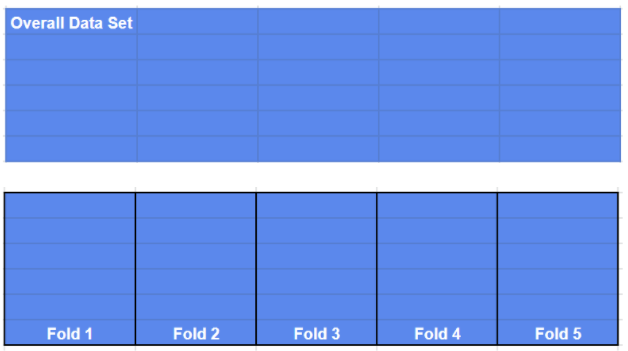
\includegraphics[scale=.6]{kfold1}\newline 
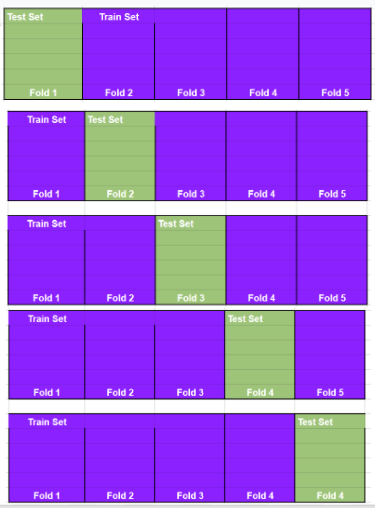
\includegraphics[scale=1]{kfold2}\newline 
\end{center}






\newpage
{\noindent}{\bf Data Sets}\newline
The following data sets were used during the classification and regression tasks for this project.\newline
{\bf Breast Cancer}\newline
Description: \newline
Task: Classification\newline
Predictor: Diagnosis (Malingant or Benign)\newline
Link:\newline \url{https://archive.ics.uci.edu/ml/datasets/Breast+Cancer+Wisconsin+%28Original%29}\newline
{\noindent}\textbf{Car Evaluation}\newline
Description:\newline
Task: Classification\newline
Predictor: Car Evaluation (Unacctable, Acctable, Good, Very Good)\newline
Link: \newline
\url{https://archive.ics.uci.edu/ml/datasets/Car+Evaluation}\\
{\noindent}\textbf{Congressional Vote}\newline
Description: 1984 United Stated Congressional Voting Records\newline
Task: Classification \newline
Predictor: Party (Reblican / Democrat) \newline
Link: \newline
\url{https://archive.ics.uci.edu/ml/datasets/Congressional+Voting+Records}\newline
{\noindent}\textbf{Albalone}\newline
Description: Physical merasurements of Albalone\newline
Task: Regression\newline
Predictor: Rings (int)\newline
Link: \newline
\url{https://archive.ics.uci.edu/ml/datasets/Abalone}\newline
{\noindent}\textbf{Computer Hardware}\newline
Description: Realative CPU performance data.\newline
Task: Regression\newline
Predictor: PRP\newline
Link: \newline
\url{https://archive.ics.uci.edu/ml/datasets/Computer+Hardware}\newline
{\noindent}\textbf{Forest Fires}\newline
Description: Forest Fire burn area data\newline
Task: Regression\newline
Predictor: Area (float)\newline
Link: \newline
\url{https://archive.ics.uci.edu/ml/datasets/Forest+Fires}\newline
	
\newpage

\section{Results}
The following results were obtained from the Classification task data sets.
Tables 1-3 display the results from the Breast Cancer, Car Evaluation and Congressional Vote data sets. These tables show the result from the train set and the test set during each fold of the \textit{k}-fold validation process. The tables also display the accuracy and error obtained during each fold, and the total accuracy and error as averaged across each of the 5 \textit{k}-folds. An accuracy(scale of 0-1) of 1 indicates that the train set had the most frequently occurring classifier equal to the most frequently occurring classifier in the test set. An error(scale of 0-1) of 0 indicates that the test set and train set had the same most frequently occurring classifier. Note in the Breast Cancer data set a value of 2 was mapped to the classifier of benign.\\ 

\begin{table}[h!]
	\begin{center}
		\caption{Breast Cancer: Naive Majority Predictor Results}
		\label{tab:table1}
		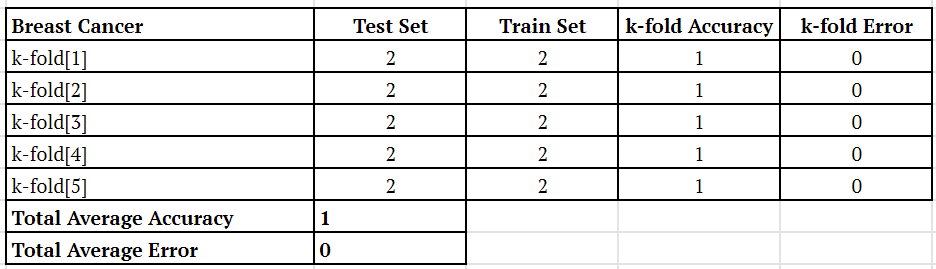
\includegraphics[scale=.6]{BC_Results}\newline
	\end{center}
\end{table}

\begin{table}[h!]
	\begin{center}
		\caption{Car Evaluation: Naive Majority Predictor Results}
		\label{tab:table2}
		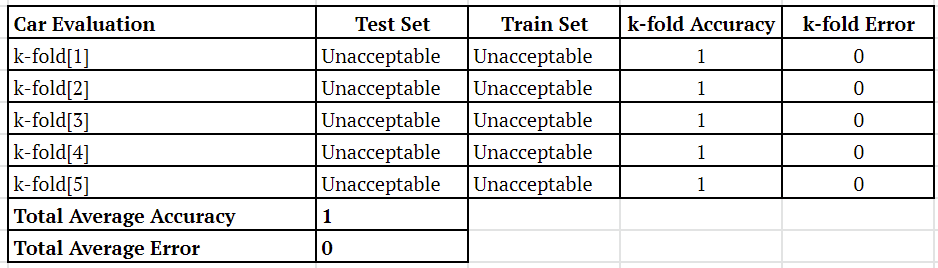
\includegraphics[scale=.6]{CE_Results}\newline
	\end{center}
\end{table}

\begin{table}[h!]
	\begin{center}
		\caption{Congressional Vote: Naive Majority Predictor Results}
		\label{tab:table3}
		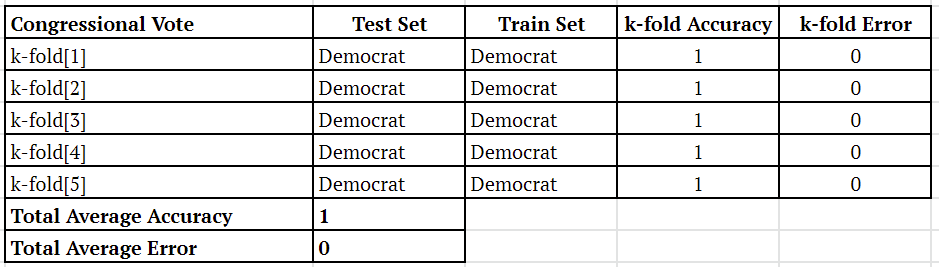
\includegraphics[scale=.6]{CV_Results}\newline
	\end{center}
\end{table}
\newpage

The following results were obtained from the Regression task data sets. Tables 4-6 display the results from the Albalone, Computer Hardware and Forest Fire data sets. These tables show the result from the train set and the test set during each fold of the \textit{k}-fold validation process.  The tables also display the error obtained during each fold, and the total error as averaged across each of the 5 \textit{k}-folds The error is the absolute error and was calculated as: $| Test Set Average - Train Set Average|$. This is meant as a measure of how far off the train set average was from the test set average. 

\begin{table}[h!]
	\begin{center}
		\caption{Albalone: Naive Mean Predictor Results}
		\label{tab:table4}
		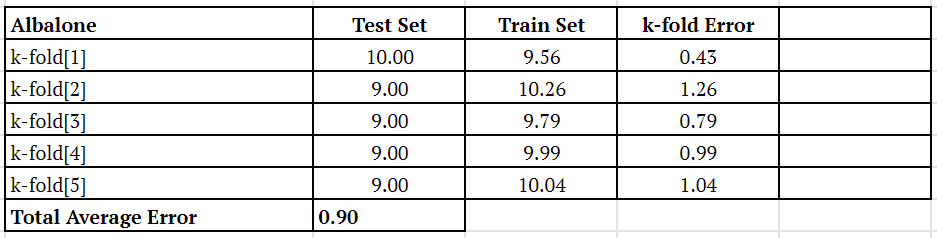
\includegraphics[scale=.6]{AB_Results}\newline
	\end{center}
\end{table}

\begin{table}[h!]
	\begin{center}
		\caption{Computer Hardware: Naive Mean Predictor Results}
		\label{tab:table5}
		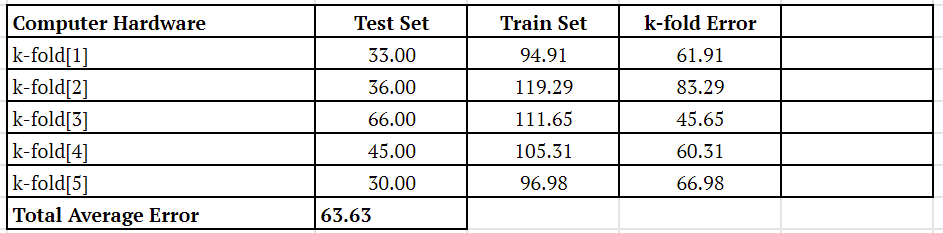
\includegraphics[scale=.6]{CH_Results}\newline
	\end{center}
\end{table}

\begin{table}[h!]
	\begin{center}
		\caption{Forest Fire: Naive Mean Predictor Results}
		\label{tab:table6}
		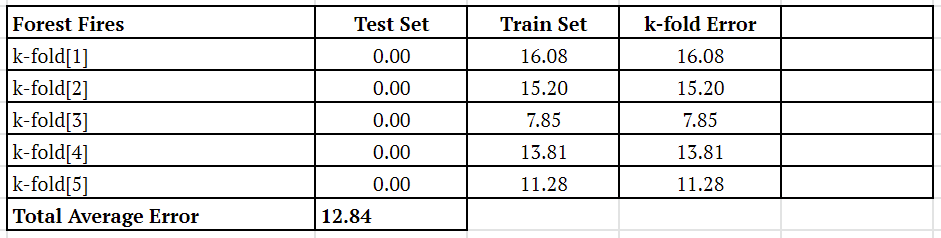
\includegraphics[scale=.6]{FF_Results}\newline
	\end{center}
\end{table}



\newpage

\section{Discussion}
The hypothesis was that since the algorithms implemented for Classification and Regression were very simplistic the prediction results from these algorithms will be highly inaccurate and produce large errors.\newline
The Classification results seemed to indicate otherwise, for all Classification data-sets run through the Naive Majority predictor, for each fold the training set matched the test set. Due to this result occurring across three different data sets, the Naive Majority predictor should under-go more review. It was validated that the test set was unique and contained no duplicate data from the train set, thus ruling out an issue in the \textit{k}-fold process it self. However, each of these data set was not shuffled prior to entering into the \textit{k}-fold generation process. It is possible that the storage structure of the data as it's pulled down raw from the source, had some intrinsic ordering that impacted the results.\newline
\hspace*{10mm}The Regression results also indicated that there was is most cases lower error than originally hypothesized. The error was relatively low \textit{k}-fold to \textit{k}-fold and on average across folds for the Albalone and Forest Fire data set. The computer hardware data-set seemed to have a larger magnitude of error. It is possible that the computer hardware had a larger spread of values in the Attribute PRP that was used to perform the Naive Average predictor on. This large spread would then transfer to the test and train sets more often. In other words, as the data get cut sliced for the test set there is a higher chance that more of the higher PRP values fall into the test set, which can attribute to the error, as the average of higher values will be higher than the average of lower values, and vice versa. The Forest Fire data set did not have a logarithmic transform applied, leading to the error being directly equal to the average that was computed by the train set. 

\section{Conclusion}
From this project it can be concluded that pre-processing the data in order to feed algorithms is an important step in Machine Learning. This project also implemented a Naive Majority and Average predictor on data sets using \textit{k}-fold cross validation. Reviewing the results, it can be seen that trends that are apparent in the raw data can have an impact on the result of our predictors. This was most noticeable in the Forest Fire data set, where many of the results were skewed towards zero. Without a logarithmic transform in place, to represent all data points from this data set on a representative scale, the overall error in our mean predictor was directly equal to the result average of our training sets. For future would it would be useful to implement a logarithmic transform of the data and in addition it would be helpful if the Naive Majority and Average predictor algorithms were improved to reduce error. 

\newpage


\end{document}